% !TeX root = ../main.tex
\chapter{Resolución numérica de ecuaciones diferenciales difusas}
\begin{chapquote}{Conversación entre Katherine Johnson \& John Glenn, \textit{Figuras ocultas}}
	John Glenn: ``Pasar de una trayectoria elíptica a otra parabólica`` \\
	Katherine Johnson: ``No se trata de una solución teórica, sino numérica`` \cite{eulernasa}
\end{chapquote}

En esta sección se van a ver diferentes técnicas para resolver ecuaciones diferenciales difusas, abarcando desde las técnicas clásicas de la resolución númerica de ecuaciones diferenciales hasta las técnicas más sofisticadas a nivel computacional.

En esta sección se va a hacer un análisis exhaustivo de las ventajas en las ventajas que nos ofrecen los distintos métodos con vistas a obtener el rendimiento más óptimo en cuánto a velocidad y en eficiencia enerǵetica.

Para entender esta sección sería conveniente revisar algunas de las técnicas mostradas en la sección anterior, y repasar las tećnicas básicas de resolución numérica de ecuaciones diferenciales difusas.

\section{El método de Euler}
En esta sección se va a desarrollar el método de Euler para problemas difusos, para ello se empieza recordando como funciona el método de Euler para ecuaciones diferenciales ordinales. Cabe recordar que este método numérico tiene orden $1$.

\subsection{Método de Euler: Versión clásica}
Se supone que se tiene un problema de valores iniciales bien definido, y lo suficiente regular para asegurar que tiene una única solución:
\[
\begin{array}{ccc}
	y'(x) & = &f(x, y)  \\
	y(x_0) & = & y_0
\end{array}.
\]
Se considera ahora una discretación del intervalo $[a, b]$ definida como:
\[
	x_i = x_0 + i h,
\]
donde $h>0$, $x_0=a$ .

El método de Euler define la siguiente solución aproximada: dada la condición inicial $y_0$
\[
	y_{i+1} = y_i + h f(x_i, y_i).
\]

\subsection{Método de Euler: Versión difusa}
Se considera el siguiente problema difuso, al que se puede dar sentido para una función f(x,y) determinista utilizando el principio de extensión de Zadeh:
\[
	\begin{array}{ccc}
		y'(x) & = &f(x, y)  \\
		y(x_0) & = & A
	\end{array},
\]
donde $A$ es un número difuso. Se supone que el problema anterior cumple el \hyperref[teorema:equivalencia]{Teorema de equivalencia entre EDO y EDD}, y se considera el problema determinista asociado:
\[
	\begin{array}{ccc}
		y' & = &f(x, y)  \\
		y(x_0) & = & a
	\end{array}
\]
donde $a \in A$. Se toma entonces $A$ como una discretización de $n+1$ elementos de $A$, donde cada elemento se denota por $a_i$, por tanto se tienen ahora $n+1$ EDO diferentes, donde cada una de estas se pueden resolver aplicando el método de Euler.
\subsection{Método de Euler: Ejemplo}
\begin{ejemplo}
Sea un problema de valores iniciales difuso:
\[
y' = 2x - 3y + 1
\]
\[
y(0) = (-1;0;1).
\]
Claramente cumple las hipótesis del \hyperref[teorema:equivalencia]{Teorema de equivalencia entre EDO y EDD}, por tanto el problema determinista asociado es:
\[
y' = 2x - 3y + 1
\]
\[
y(0) = a,
\]
con $a \in [-1, 1]$. \\
En primer lugar, hay que discretizar el intervalo $[-1, 1]$, para ello, fijamos m>0 y para cada $i=0...m-1$ se considera una partición dada por:
\[
a_i = -1 + \frac{2i}{m-1}.
\]
Teniendo en cuenta estas particiones, se puede aproximar la solución del problema difuso resolviendo las $m$ ecuaciones diferenciales que se deducen al tomar:
\[
y' = 2x - 3y + 1
\]
\[
y(0) = a_i.
\]
Se construye ahora el método de Euler para la ecuación asociada a $a_i$ con tamaño del paso $h$, sea $x_0=0$ y tomemos $y_0 = a_i$, siguiendo entonces con le definición del método nos queda:
\[
y_{j+1} = y_j + h (2x_j - 3y_j + 1)
\]
\[
x_{j+1} = x_0 + hj.
\]

Para comparar el error de nuestro método, tengamos en cuenta que la solución exacta de la ecuación diferencial con dato inical $a_i$ es:
\[
y_i(x) = \frac{e^{-3 x} (-1 + 9 a_i + e^{3 x}(1 + 6 x))}{9}
\]
A continuación, se ofrecerán varías implementaciones del método con información descriptiva acerca del rendimiento energético y en tiempo:

\subsection{Experimentos numéricos}
Se va a tratar de resolver el problema anterior aplicando el método de Euler, con una implementación en C y otra en Python, donde se varía la cantidad de particiones del número difuso triangular y con 100 pasos en el método de Euler.
\subsubsection{Implementación en Python}
\begin{figure}[H]
	\frame{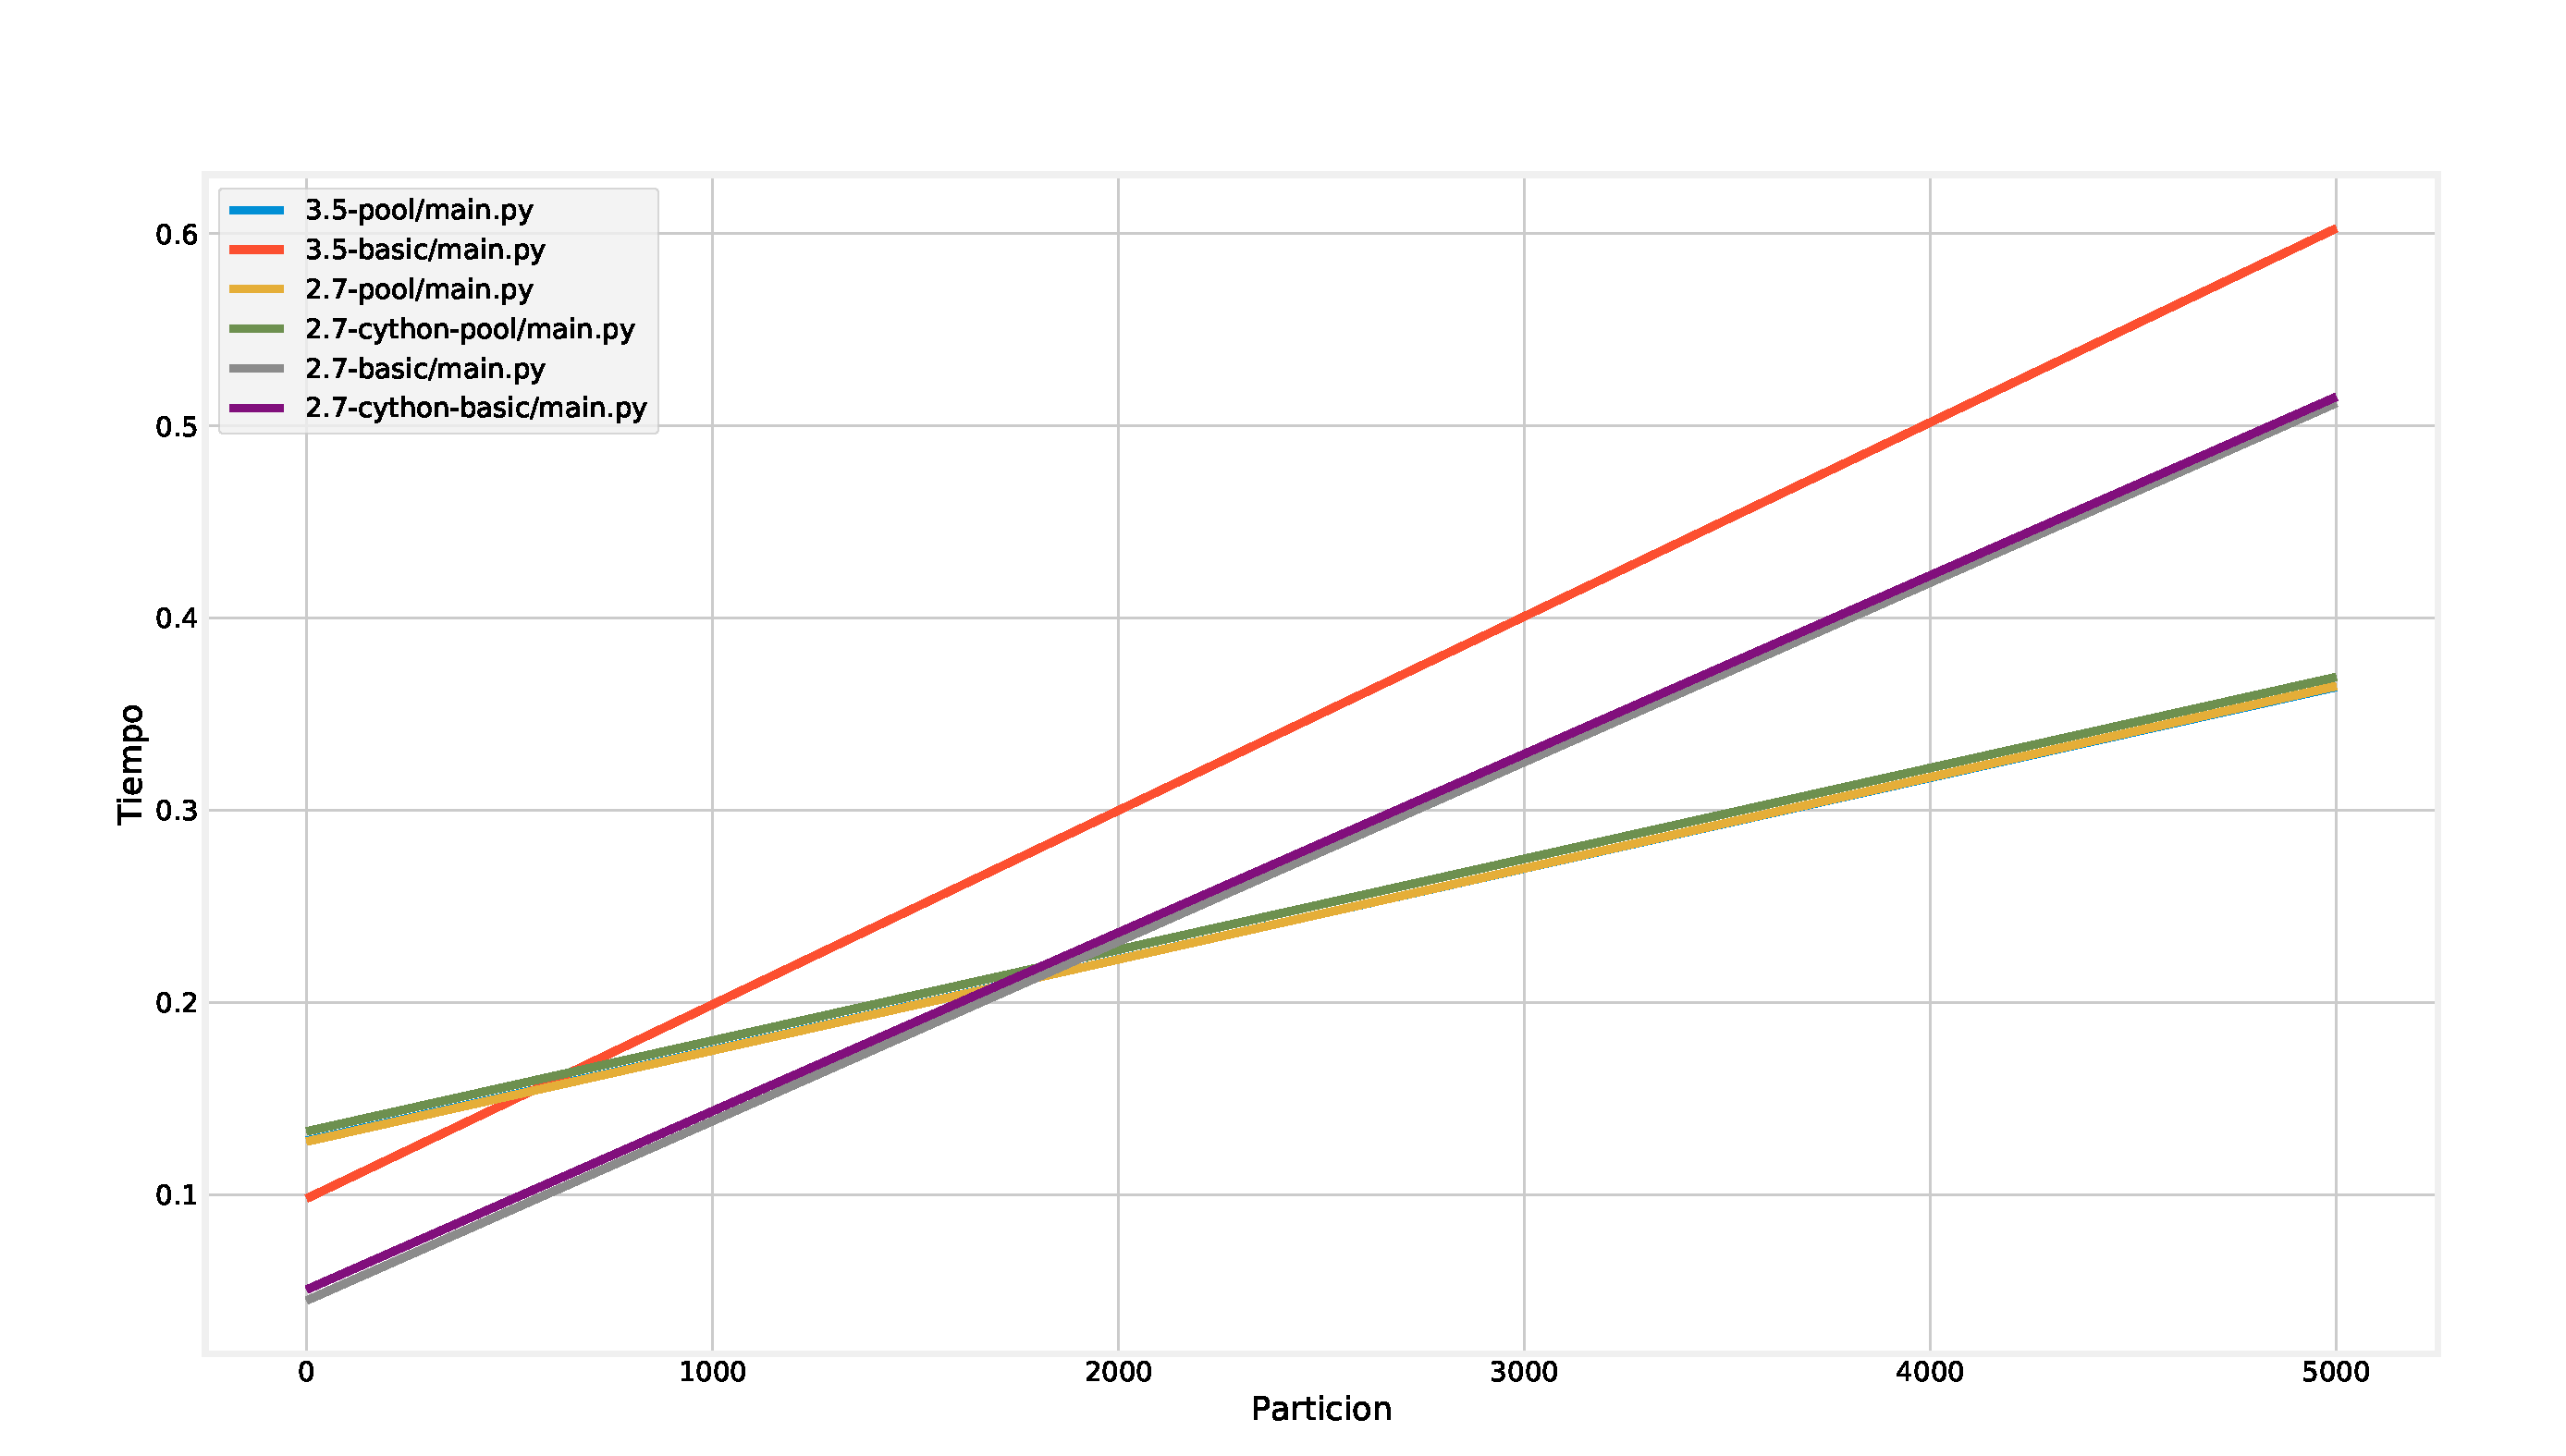
\includegraphics[width=\textwidth]{grafica_python_euler_comparativa.pdf}}
	\centering
	\caption{Distintos resultados en Python}
	\label{fig:eulerpython}
\end{figure}

Se pueden observar, varios patrones:

\begin{itemize}
	\item La forma menos eficiente de resolver el problema es usando una versión más reciente de Python.
	\item Trabajar con Cython no nos asegura un rendimiento mejor.
	\item El crecimiento del tiempo de ejecución en paralelo crece mucho menor que en secuencial.
	\item Si se quiere resolver un problema pequeño $(n < 2000)$ es conveniente hacerlo de manera secuencial.
\end{itemize}

A continuación, se muestra una tabla con los resultados obtenidos por cada test.
\begin{table}[H]
	\centering
	\begin{tabular}{|c|c|}
		\hline
		\textbf{Test}  & \textbf{Tiempo}        \\ \hline
		2.7 Paralelo   & 61 minutos    \\
		3.5 Paralelo   & 61 minutos   \\
		2.7 Cython     & 85 minutos    \\
		2.7 Secuencial & 85.22 minutos \\ 
		3.5 Secuencial & 100 minutos   \\
		\hline
	\end{tabular}%
\end{table}
\subsubsection{Implementación en C: Secuencial}
\begin{figure}[H]
	\frame{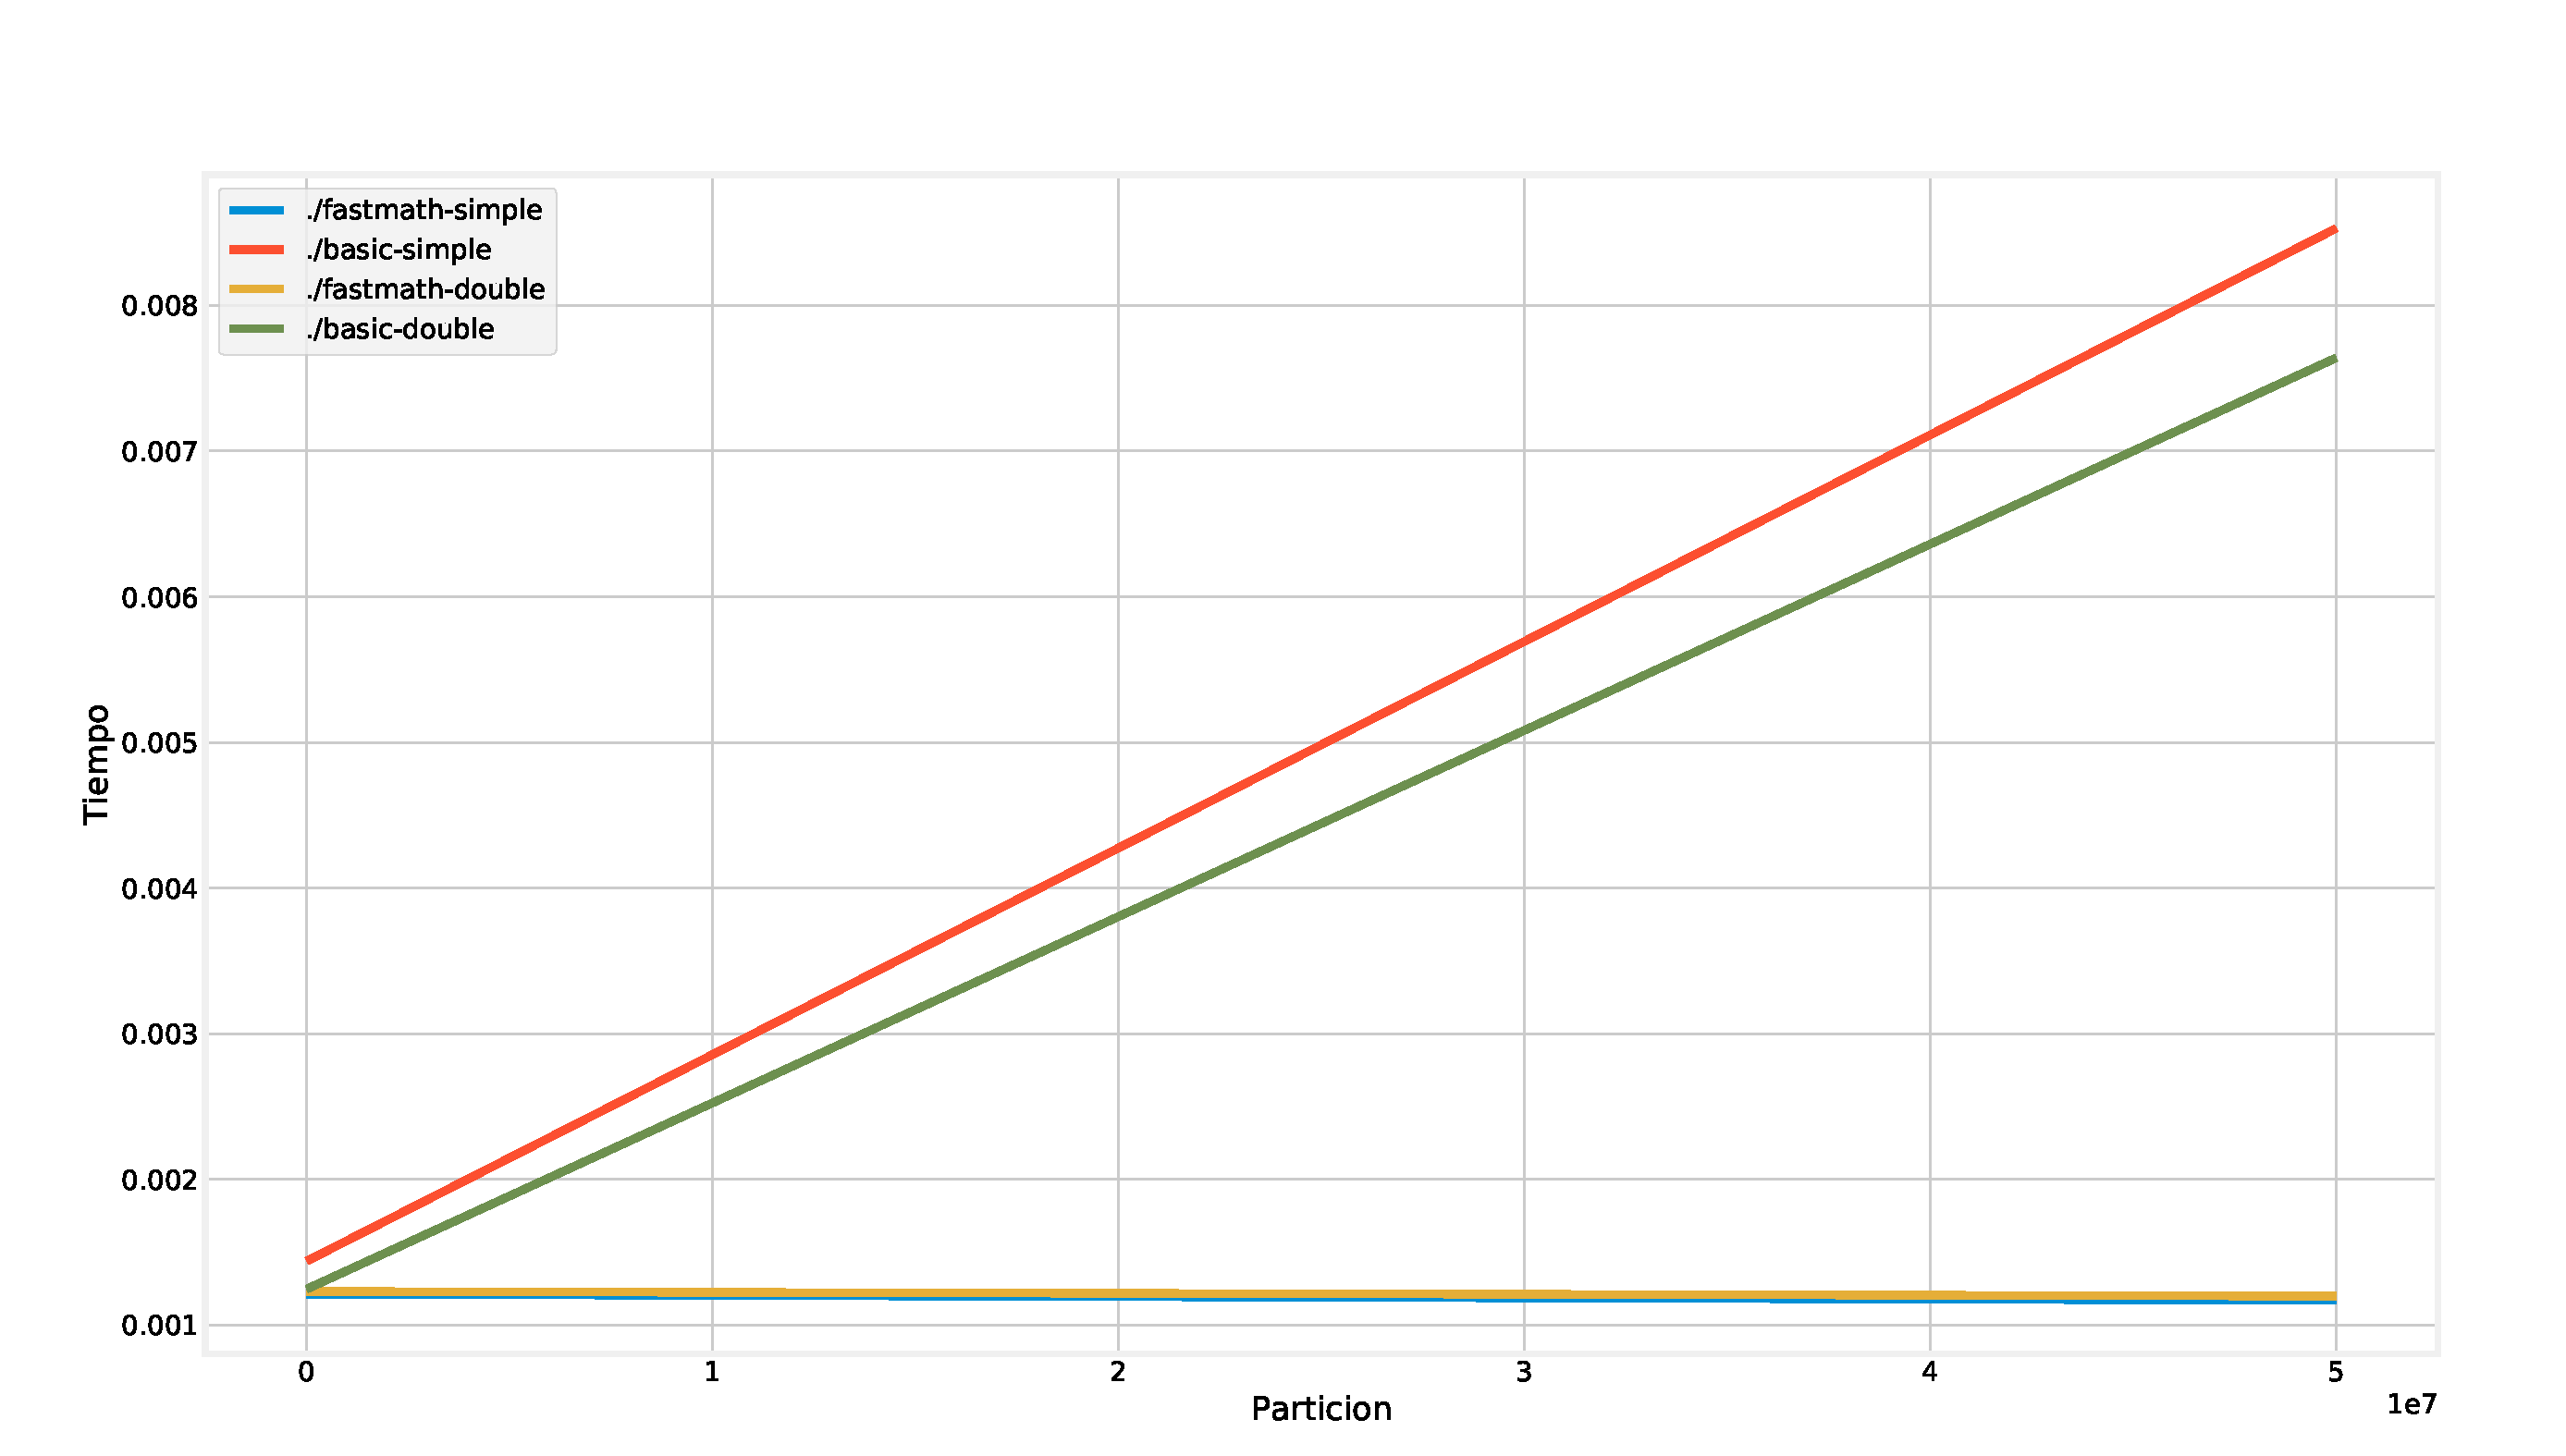
\includegraphics[width=\textwidth]{grafica_cseq_euler_comparativa.pdf}}
	\centering
	\caption{Distintos resultados en C}
	\label{fig:eulercseq}
\end{figure}
En esta parte se va a probar una implementación en C, usando diferentes técnicas numéricas.
\begin{itemize}
	\item Se han obtenido resultados esperados en las compilaciones básicas de los programas.
	\item Cuando se trabaja en doble precisión, el rendimiento se reduce, pero en C se siguen consiguiendo resultados bastantes rápidos independientemente de la precisión.
	\item El consumo de RAM es bastante reducido.
	\item El procesador al ser un procesador de 64 bits, trabaja mejor en doble precisión que en simple precisión.
\end{itemize}

A continuación, se muestra una tabla con los resultados obtenidos por cada test.

\begin{table}[H]
	\centering
	\begin{tabular}{|c|c|}
		\hline
		\textbf{Test}  & \textbf{Tiempo}        \\ \hline
		Fastmath simple precisión & 11.9 segundos \\ 
		Fastmath doble precisión  & 12.15 segundos    \\
		Doble precisión  & 75.80 segundos \\
		Simple precisión    & 85 segundos    \\
		\hline
	\end{tabular}%
\end{table}

Ahora vamos a ver que sucede si también se aumenta el número de particiones para representar el número difuso, y para obtener resultados más interesantes, se van a empezar las iteraciones en 10000.

\begin{figure}[H]
	\frame{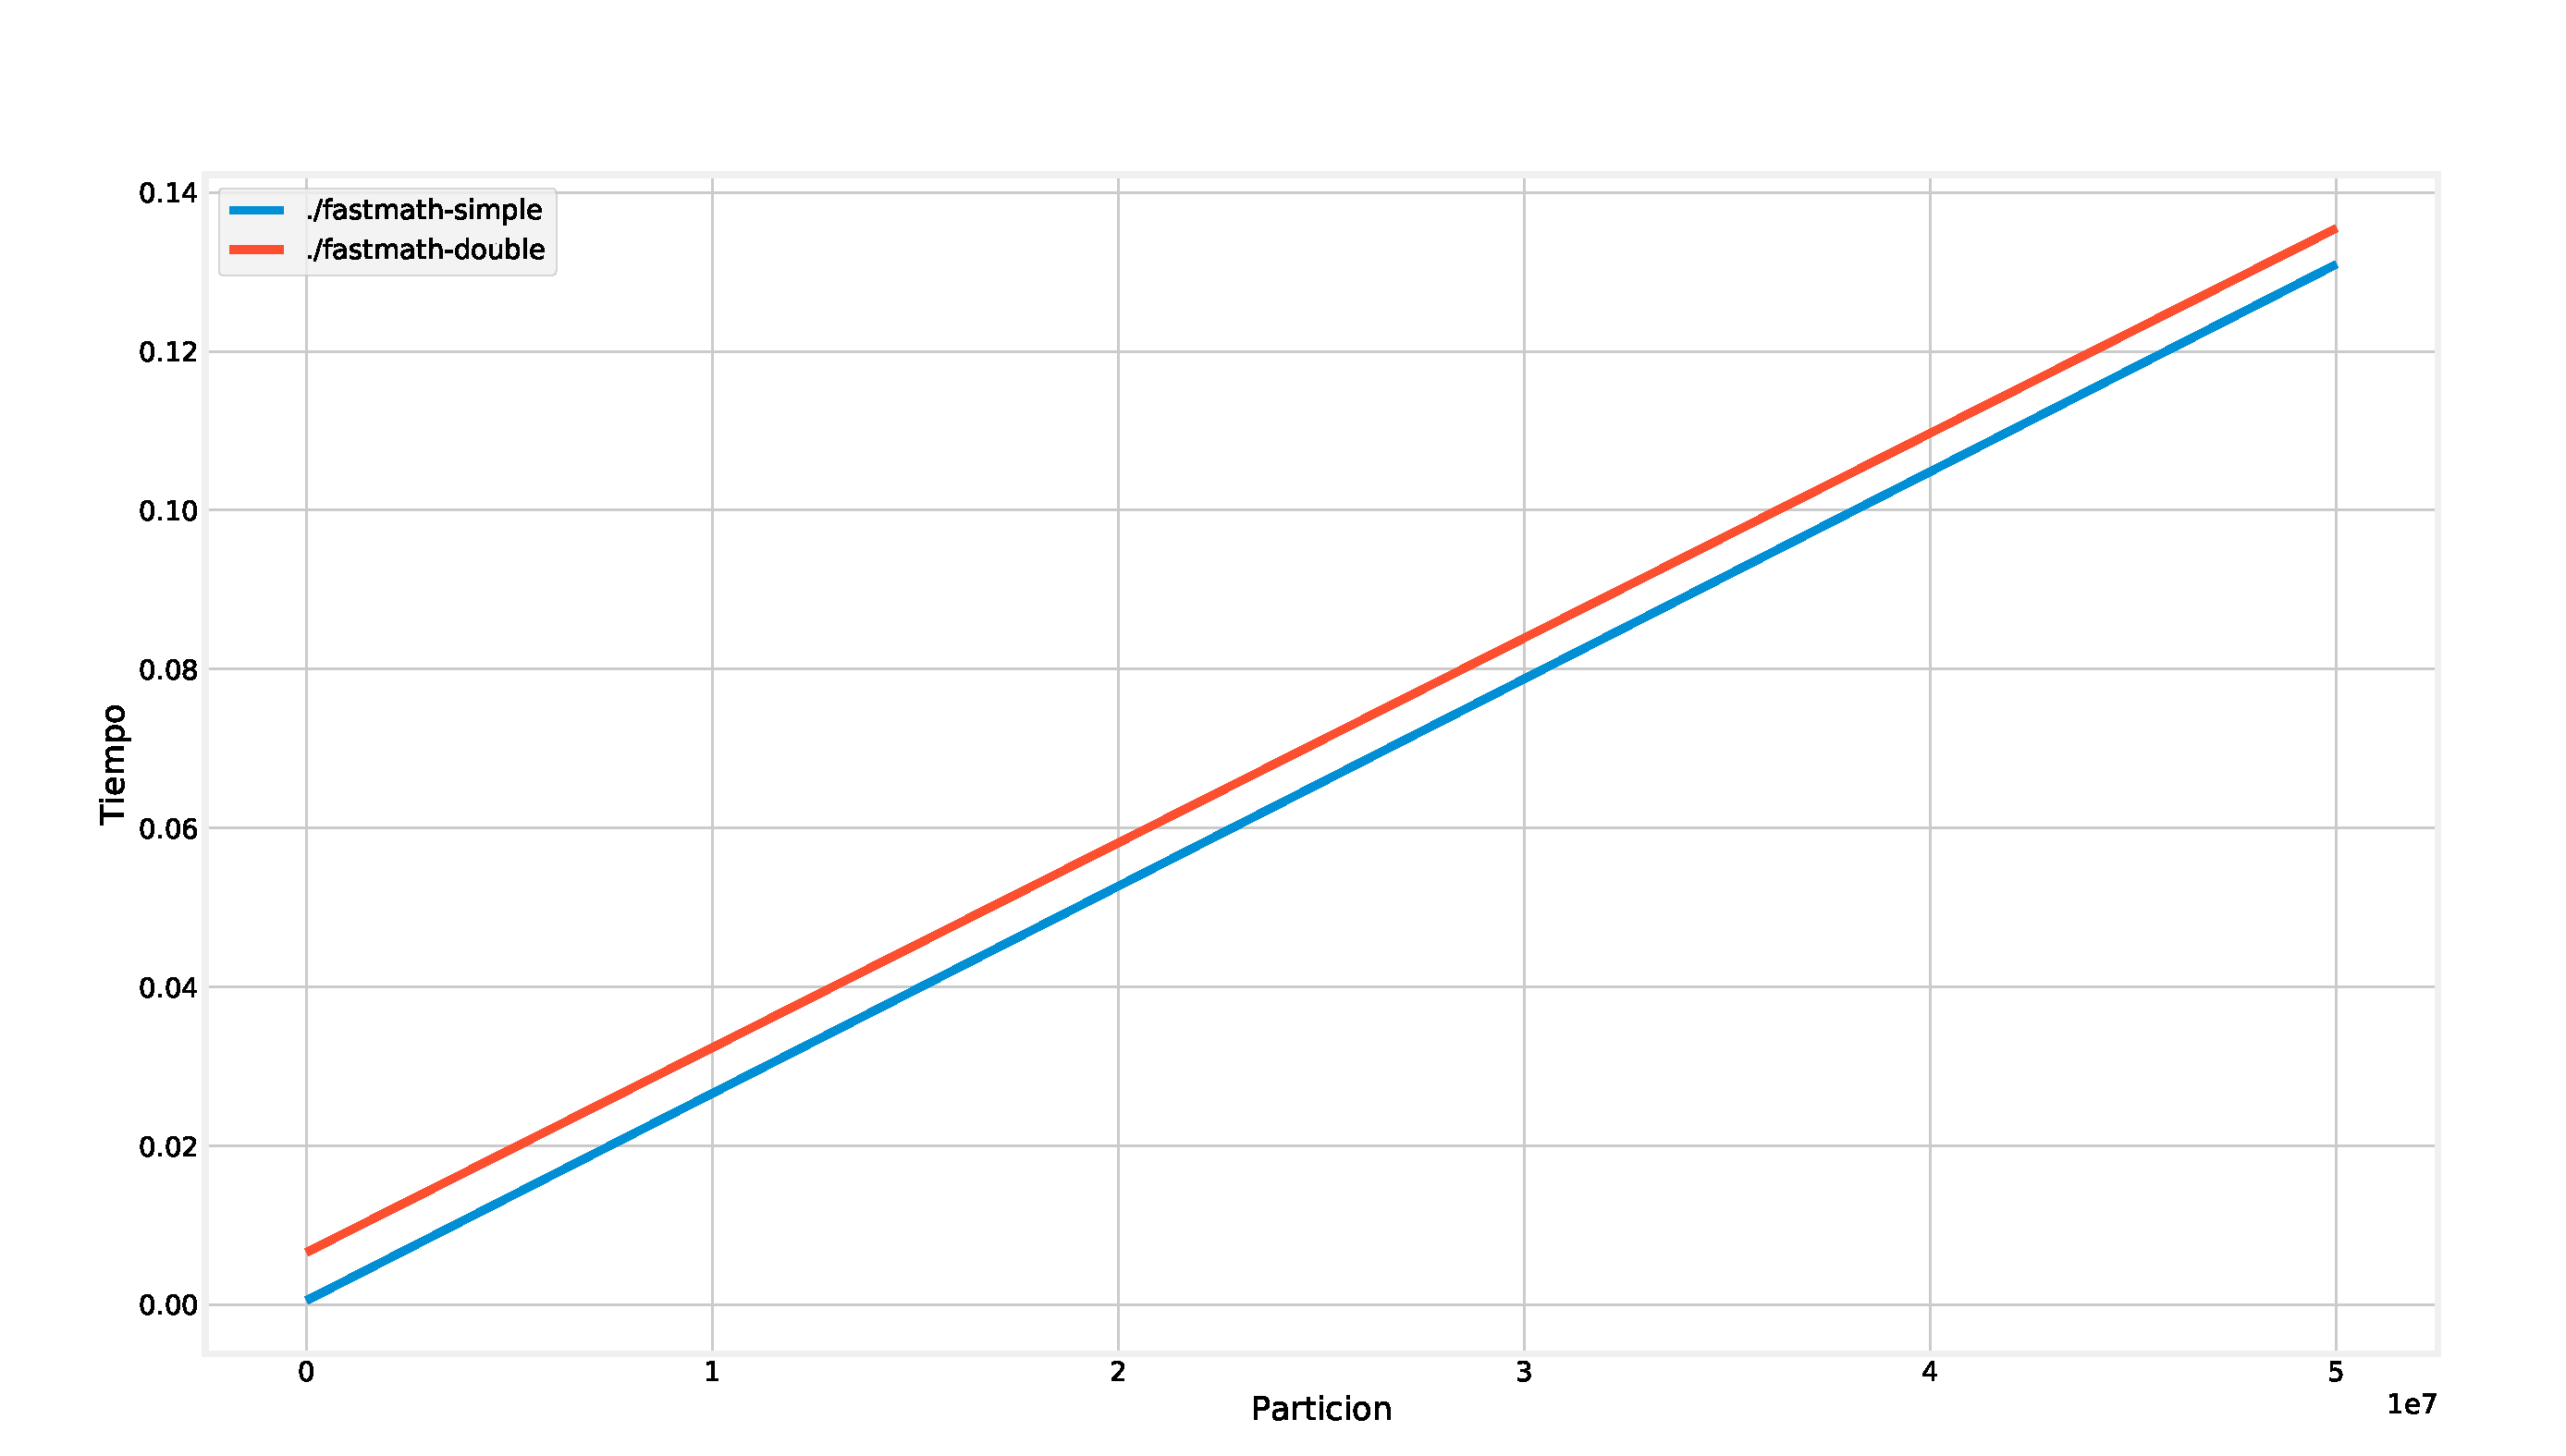
\includegraphics[width=\textwidth]{grafica_cseq_euler_comparativa_2.pdf}}
	\centering
	\caption{Distintos resultados en C}
	\label{fig:eulercseq2}
\end{figure}
Aquí se pueden sacar una conclusiones diferentes,
\begin{enumerate}
	\item Es más óptimo trabajar en simple precisión con fastmath.
	
	\item Pese a todo, aunque se esté haciendo $10^{16}$ iteraciones, el algoritmo tarda como mucho $0.25$ segundos, aún no es necesario plantearse trabajar en paralelo.
\end{enumerate}
Finalmente, se introduce una tabla con los tiempos de cada prueba

\begin{table}[H]
	\centering
	\begin{tabular}{|c|c|}
		\hline
		\textbf{Test}  & \textbf{Tiempo}        \\ \hline
		Fastmath simple precisión & 1278.03 segundos \\ 
		Fastmath doble precisión  & 1341.10 segundos  \\ \hline
	\end{tabular}%
\end{table}

Por otro lado, en la siguiente tabla se muestran los consumo energético de los distintos ejemplos para $10^{5}$ iteraciones.

\begin{table}[H]
	\centering
	\begin{tabular}{|c|c|}
		\hline
		\textbf{Test}  & \textbf{Consumo energético}        \\ \hline
		Fastmath simple precisión & $118.644028 \mu A/s$ \\ 
		Fastmath doble precisión  & $118.644058 \mu A/s$ \\
		Simple precisión & $ 152.542389 \mu A/s$ \\
		Doble precisión & $ 169.491638 \mu A/s$ \\
		\hline
	\end{tabular}%
\end{table}
\subsubsection{Conclusiones}
En contra de lo que se pueda pensar comúnmente, trabajar con precisión doble es más eficiente en procesadores modernos de 64 bits que trabajar en precisión simple, así que no hay que tener miedo a trabajar con doble precisión. \\
Los resultados obtenidos en C con la flag -OFast son sorprendentes, tan sorprendentes que no se ha planteado la necesidad  de implementar el método en paralelo por la eficiencia de aplicar esa flag.
\\
Y no sólo permite obtener una solución numérica más rápidamente, sino que permite consumir menos recursos energéticos, lo que se traduce en un ahorro económico a la hora de trabajar a una escala mayor, y un menor impacto medioambiental, por tanto utilizar la flag -Ofast al compilar es la mejor opción en todos los aspectos
\end{ejemplo}

\section{Método de Runge-Kutta de cuarto orden}
Por otro lado, vamos a desarrollar el método de Runge Kutta. Como es sabido el orden de convergencia de este método es mayor que el de Euler, por lo que se esperan mejores resultados a priori.

\subsection{Método de Runge-Kutta de cuarto orden: Versión clásica}
Se supone que se tiene un problema de valores iniciales bien definido, y lo suficiente regular para asegurar que tiene soluciones:
\[
\begin{array}{ccc}
y'(x) & = &f(x, y)  \\
y(x_0) & = & y_0
\end{array}.
\]
Como en el método de Euler, lo que se busca primer lugar es una discretización del intervalo $[x_0, x_f]$, se supone que se quiere discretizar el intervalo en $n$ valores, sea entonces:
\[
	h = \frac{x_f - x_0}{n}.
\]
Por tanto, podemos definir 
\[
	x_i = x_0 + i h.
\]
Por otro lado, el paso iterativo sobre $y_{i+1}$ viene dado por:
\[
	y_{i+1} = y_i + \frac{h}{6} (k_1 + 2k_2 + 2k_3 + k_4),
\]
donde se definen:
\[
\begin{array}{ccc}
	k_1 & = & f(x_i, y_i) \\
	k_2 & = & f\left(x_i + \frac{h}{2}, y_i + \frac{k_1 h}{2}\right) \\
	k_3 & = & f\left(x_i + \frac{h}{2}, y_i + \frac{k_2 h}{2}\right) \\
	k_4 & = & f(x_i + h, y_i + k_3 h)
\end{array}
\]

\subsection{Método de Runge-Kutta de cuarto orden: Versión difusa}
Se considera el siguiente problema difuso, en el sentido del principio de extensión de Zadeh
\[
\begin{array}{ccc}
y' & = &f(x, y)  \\
y(x_0) & = & A
\end{array},
\]
donde $A$ es un número difuso. Se toma entonces que el problema anterior cumple el \hyperref[teorema:equivalencia]{Teorema de equivalencia entre EDO y EDD}, y se considera el problema determinista asociado:
\[
\begin{array}{ccc}
y' & = &f(x, y)  \\
y(x_0) & = & a
\end{array},
\]
donde $a \in A$, se toma entonces $A$ como una discretización de $n+1$ elementos de $A$, donde cada elemento se denota por $a_i$, por tanto se tienen ahora $n+1$ EDO diferentes, donde cada una de estas se pueden resolver aplicando el método de Método de Runge-Kutta de cuarto orden.

\subsection{Método de Runge-Kutta de cuarto orden: Ejemplo}
Para poder comparar correctamente los distintos métodos vamos a implementar el mismo problema usando el método de Runge-Kutta.

\subsection{Experimentos numéricos}
Se va a tratar de resolver el problema anterior aplicando el método de Runge-Kutta, con una implementación en C, donde se varía la cantidad de particiones del número difuso triangular, y con 100 pasos en el método de Euler.

\begin{figure}[H]
	\frame{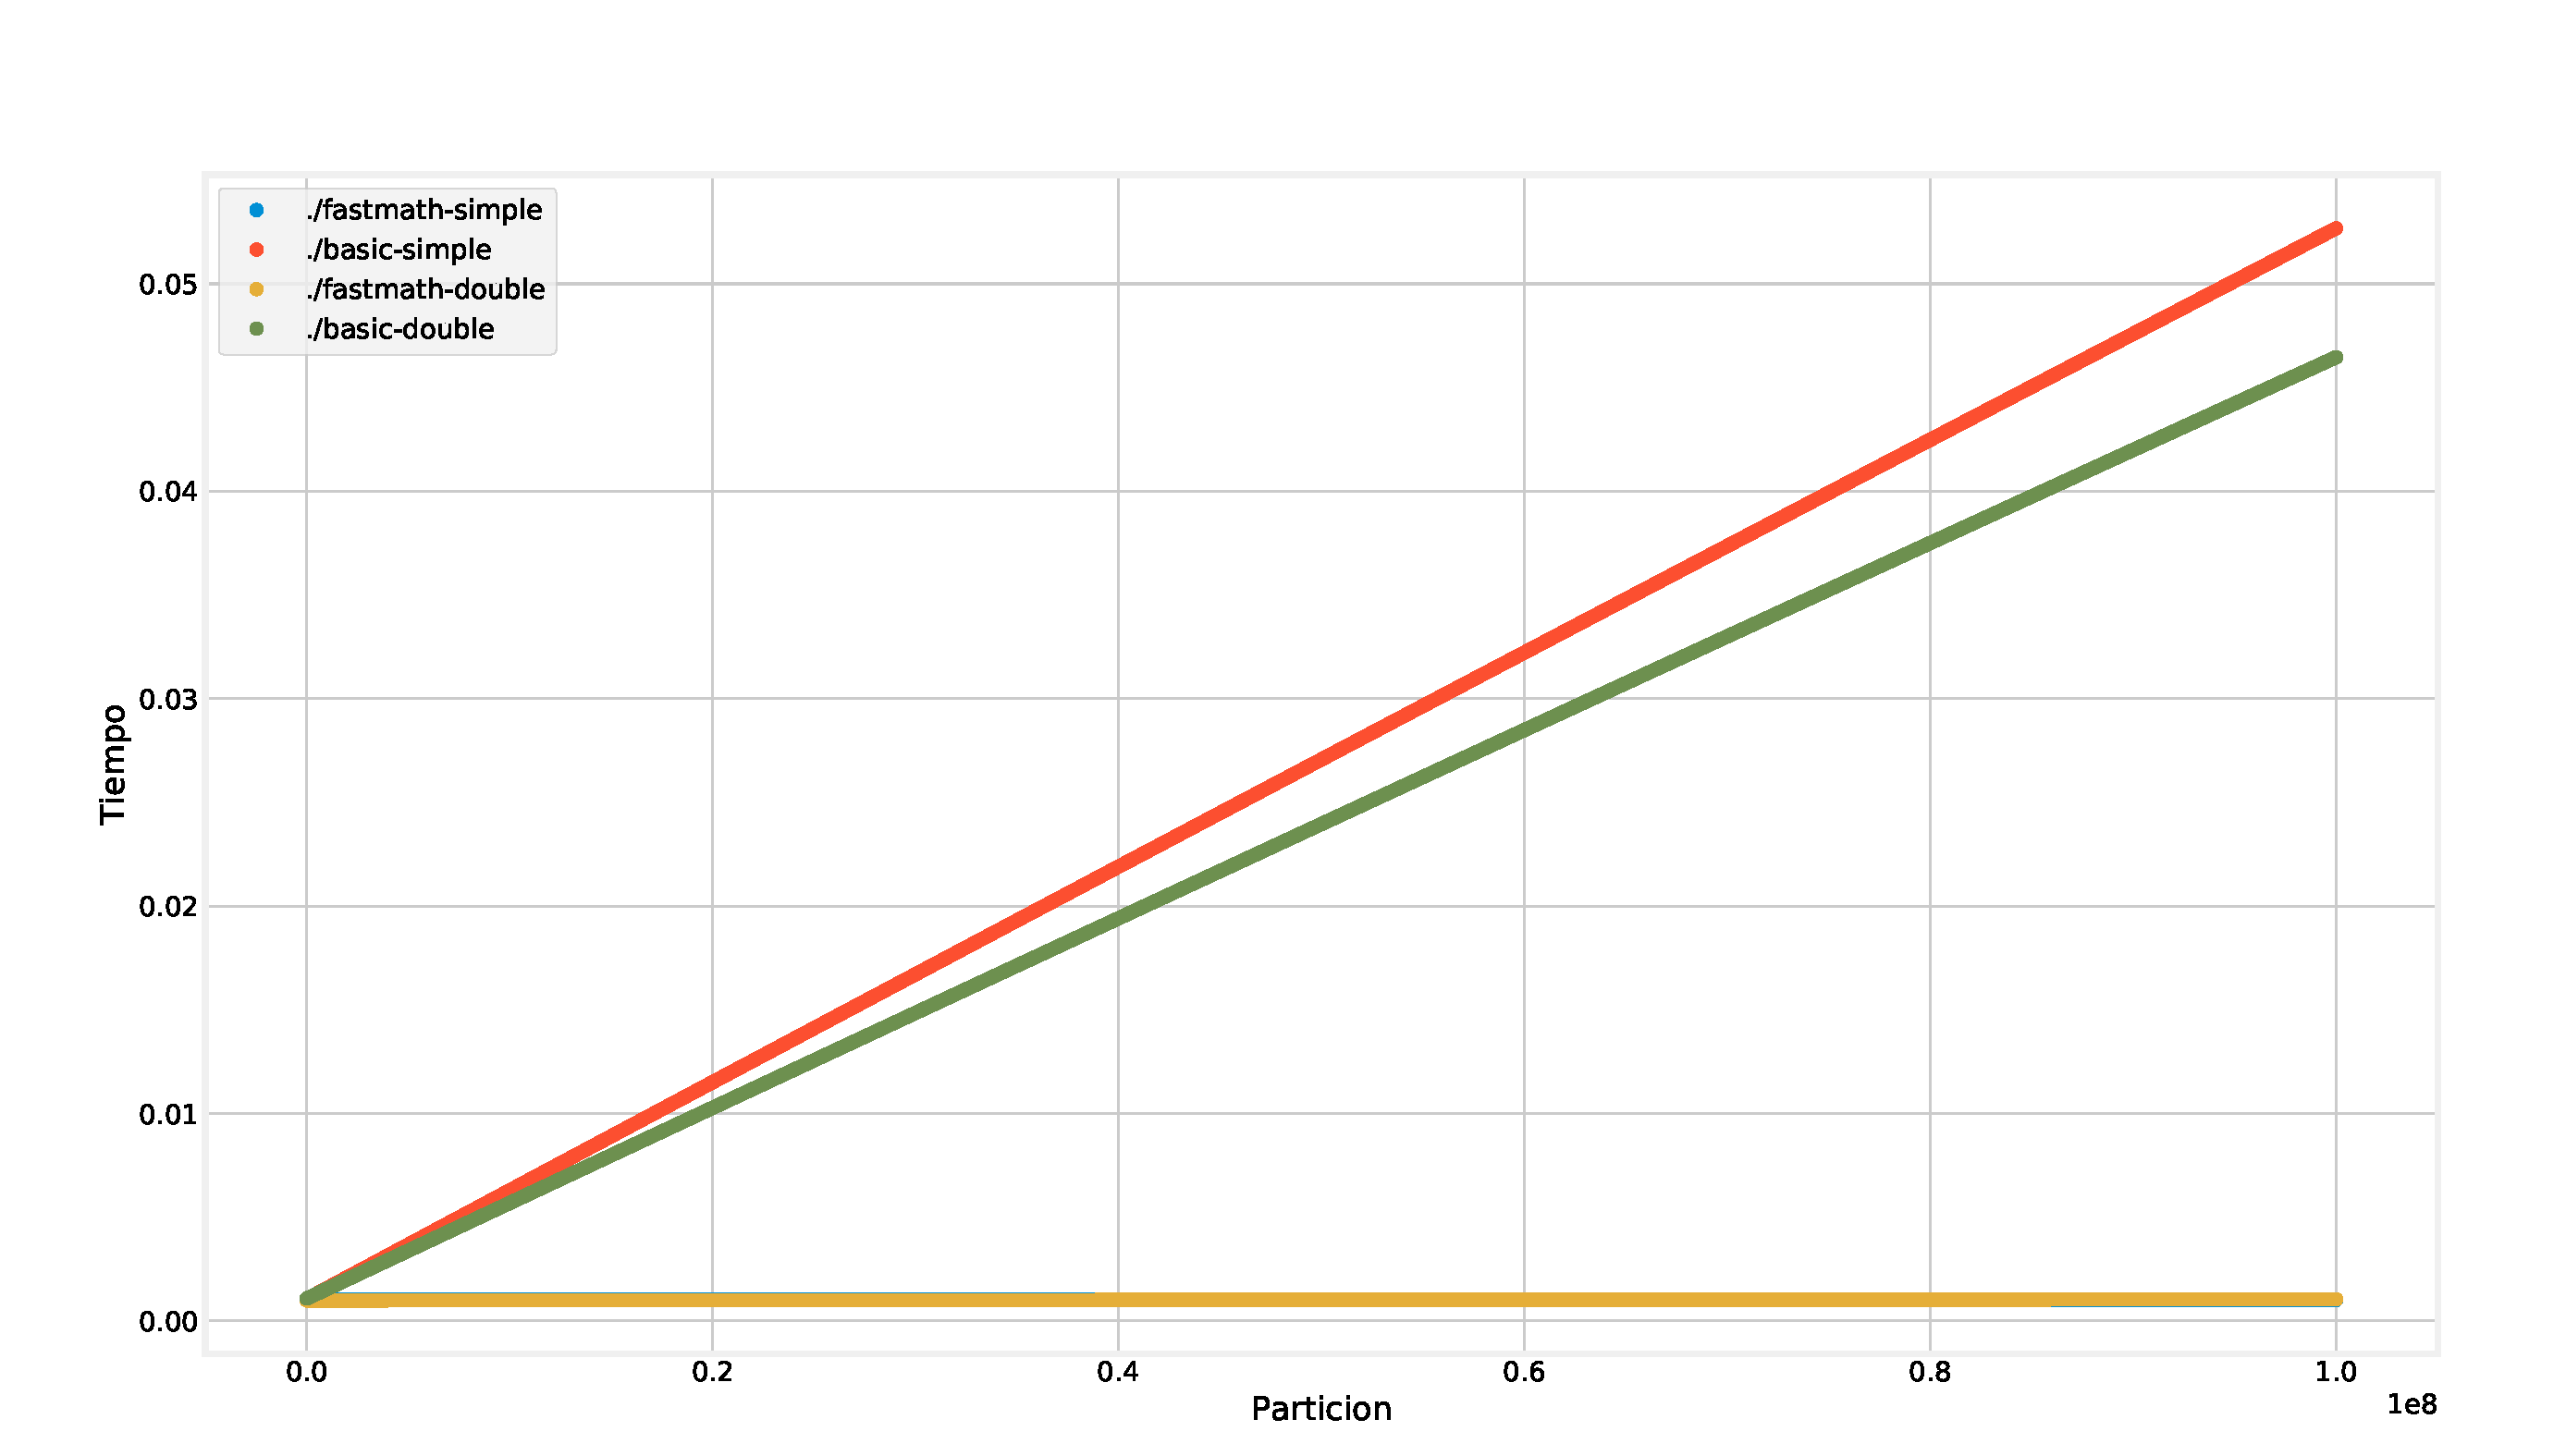
\includegraphics[width=\textwidth]{grafica_cseq_rk_comparativa.pdf}}
	\centering
	\caption{Distintos resultados en C}
	\label{fig:rungekuttacseq}
\end{figure}

\begin{table}[H]
	\centering
	\begin{tabular}{|c|c|}
		\hline
		\textbf{Test}  & \textbf{Tiempo}        \\ \hline
		Fastmath simple precisión   & 10.1921305656 segundos    \\
		Fastmath doble precisión  & 10.1441464424 segundos   \\
		Basic doble precisión  &238.943392515 segundos    \\
	    Basic simple precisión & 270.01487565 segundos \\ 
		\hline
	\end{tabular}%
\end{table}

\section{Comparativas}
Si se observa la tabla de tiempos del algoritmo de Euler respecto del algoritmo de Runge-Kutta se pueden encontrar una serie de informaciones interesante:

\begin{itemize}
	\item Los modos básicos son más rápidos en el método de Euler, también tiene más sentido, pues en el método de Runge-Kutta necesita de más operaciones.
	
	\item Aunque Runge-Kutta precise de más operaciones, Runge Kutta tiene un mayor orden de convergencia.
	
	\item Al introducir la flag -Ofast el compilador optimiza Runge-Kutta lo suficiente como para poder afirmar que en este caso, Runge-Kutta es más rápido que el método de Euler, y además tiene un mayor orden de convergencia, por tanto, el mejor método en todos los aspectos es aparentemente el método de Runge-Kutta con la flag -ofast.
\end{itemize}

\section{Método difuso paralelizado}
Los dos métodos estudiados anteriormente se pueden resumir, de la siguiente forma:
\begin{itemize}
	\item Se parte de una función determinista y se considera la ecuación difusa asociada a ella mediante el principio de extensión
		
	\item Se considera una discretización del número difuso.
	
	\item Se resuelve numéricamente para cada uno de los valores que se encuentra en la discretización.
\end{itemize}
Se observa, que el último paso es independiente para cada valor discretizado del número difuso, por tanto, se podría paralelizar el algoritmo anterior de manera que cada ecuación diferencial se resuelve al mismo tiempo de forma paralela, esto es útil si se quiere hacer una discretización muy fina del número difuso, podemos ver una implementación en \ref{prueba:cuda}